\element{mob}{
\begin{question}{mob 01}
Soit le schéma suivant. Donner la mobilité du mécanisme.
\begin{center}
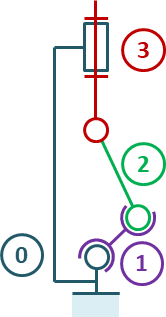
\includegraphics[width=3cm]{cas_01}
\end{center}
	\begin{reponses}	
	\bonne 2
	\mauvaise 0
	\mauvaise 1
	\mauvaise 3
	\end{reponses}
\end{question}\\}

\element{mob}{
\begin{question}{mob 02}
Soit le schéma suivant. Donner la mobilité du mécanisme.
\begin{center}
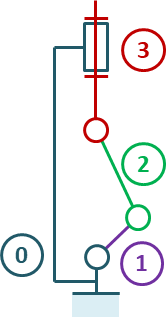
\includegraphics[width=3cm]{cas_02}
\end{center}
	\begin{reponses}	
	\bonne 0
	\mauvaise 1
	\mauvaise 2
	\mauvaise 3
	\end{reponses}
\end{question}\\}


\element{mob}{
\begin{question}{mob 03}
Soit le schéma suivant. Donner la mobilité du mécanisme.
\begin{center}
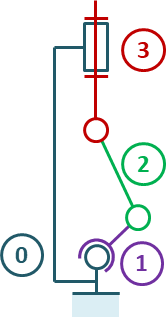
\includegraphics[width=3cm]{cas_03}
\end{center}
	\begin{reponses}	
	\bonne 1
	\mauvaise 0
	\mauvaise 2
	\mauvaise 3
	\end{reponses}
\end{question}\\}


\element{mob}{
\begin{question}{mob 04}
Soit le schéma suivant. Donner la mobilité du mécanisme.
\begin{center}
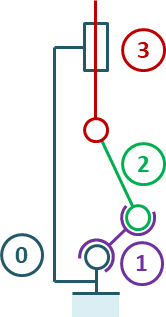
\includegraphics[width=3cm]{cas_04}
\end{center}
	\begin{reponses}	
	\bonne 3
	\mauvaise 0
	\mauvaise 1
	\mauvaise 2
	\end{reponses}
\end{question}\\}

\element{mob}{
 \begin{question}{mob 05}
 Soit le schéma suivant. Donner la mobilité du mécanisme.
 \begin{center}
 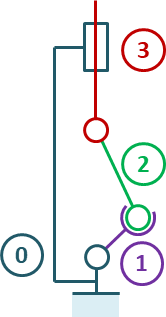
\includegraphics[width=3cm]{cas_05}
 \end{center}
	 \begin{reponses}	
	 \bonne 2
	 \mauvaise 0
	 \mauvaise 1
	 \mauvaise 3
	 \end{reponses}
 \end{question}\\}


\element{mob}{
\begin{question}{mob 06}
Soit le schéma suivant. Donner la mobilité du mécanisme.
\begin{center}
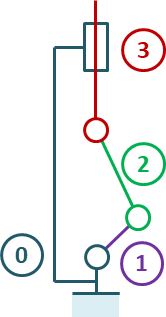
\includegraphics[width=3cm]{cas_06}
\end{center}
	\begin{reponses}	
	\bonne 1
	\mauvaise 0
	\mauvaise 2
	\mauvaise 3
	\end{reponses}
\end{question}\\}

\element{mob}{
\begin{question}{mob 07}
Soit le schéma suivant. Donner la mobilité du mécanisme.
\begin{center}
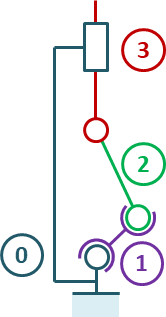
\includegraphics[width=3cm]{cas_07}
\end{center}
	\begin{reponses}	
	\bonne 2
	\mauvaise 0
	\mauvaise 1
	\mauvaise 3
	\end{reponses}
\end{question}\\}

\element{mob}{
\begin{question}{mob 08}
Soit le schéma suivant. Donner la mobilité du mécanisme.
\begin{center}
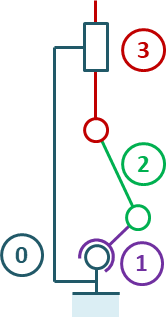
\includegraphics[width=3cm]{cas_08}
\end{center}
	\begin{reponses}	
	\bonne 1
	\mauvaise 0
	\mauvaise 2
	\mauvaise 3
	\end{reponses}
\end{question}\\}


\element{mob}{
\begin{question}{mob 09}
Soit le schéma suivant. Donner la mobilité du mécanisme.
\begin{center}
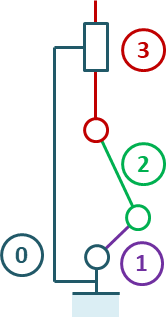
\includegraphics[width=3cm]{cas_09}
\end{center}
	\begin{reponses}	
	\bonne 1
	\mauvaise 0
	\mauvaise 3
	\mauvaise 2
	\end{reponses}
\end{question}\\}


\element{mob}{
\begin{question}{mob 10}
Soit le schéma suivant. Donner la mobilité du mécanisme.
\begin{center}
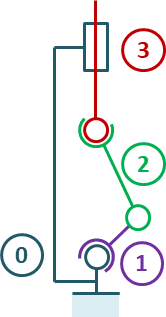
\includegraphics[width=3cm]{cas_10}
\end{center}
	\begin{reponses}	
	\bonne 3
	\mauvaise 0
	\mauvaise 1
	\mauvaise 2
	\end{reponses}
\end{question}\\}


\element{mob}{
\begin{question}{mob 11}
Soit le schéma suivant. Donner la mobilité du mécanisme.
\begin{center}
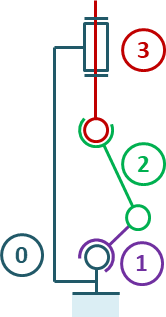
\includegraphics[width=3cm]{cas_11}
\end{center}
	\begin{reponses}	
	\bonne 2
	\mauvaise 0
	\mauvaise 1
	\mauvaise 3
	\end{reponses}
\end{question}\\}

\element{mob}{
\begin{question}{mob 12}
Soit le schéma suivant. Donner la mobilité du mécanisme.
\begin{center}
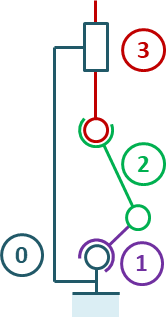
\includegraphics[width=3cm]{cas_12}
\end{center}
	\begin{reponses}	
	\bonne 2
	\mauvaise 0
	\mauvaise 1
	\mauvaise 3
	\end{reponses}
\end{question}\\}

\element{mob2}{
\begin{question}{mob2 1}
Soit le schéma suivant. Donner la mobilité du mécanisme.
\begin{center}
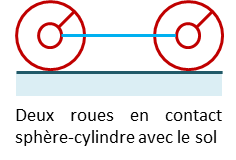
\includegraphics[width=5cm]{exo_01}
\end{center}
	\begin{reponses}	
	\bonne 6
	\mauvaise 0
	\mauvaise 1
	\mauvaise 2
	\mauvaise 3
	\mauvaise 4
	\mauvaise 5
	\end{reponses}
\end{question}\\}

\element{mob2}{
\begin{question}{mob2 2}
Soit le schéma suivant. Donner la mobilité du mécanisme.
\begin{center}
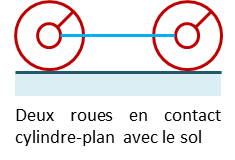
\includegraphics[width=5cm]{exo_02}
\end{center}
	\begin{reponses}	
	\bonne 5
	\mauvaise 0
	\mauvaise 1
	\mauvaise 2
	\mauvaise 3
	\mauvaise 4
	\mauvaise 6
	\end{reponses}
\end{question}\\}

\element{mob2}{
\begin{question}{mob2 3}
Soit le schéma suivant. Donner la mobilité du mécanisme.
\begin{center}
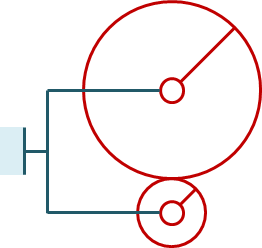
\includegraphics[width=5cm]{exo_03}
\end{center}
	\begin{reponses}	
	\bonne 2
	\mauvaise 0
	\mauvaise 1
	\mauvaise 5
	\mauvaise 3
	\mauvaise 4
	\mauvaise 6
	\end{reponses}
\end{question}\\}

\element{mob2}{
\begin{question}{mob2 4}
Soit le schéma suivant. Donner la mobilité du mécanisme.
\begin{center}
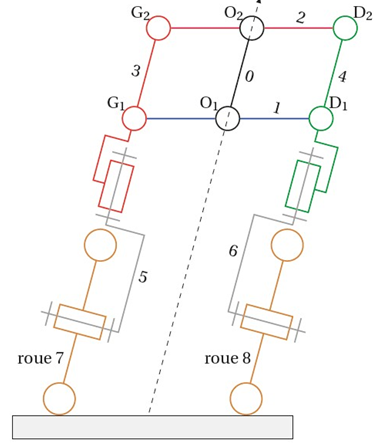
\includegraphics[width=5cm]{exo_04}
\end{center}
	\begin{reponses}	
	\bonne 9
	\mauvaise 1
	\mauvaise 3
	\mauvaise 5
	\mauvaise 7
	\mauvaise 2
	\mauvaise 4
	\end{reponses}
\end{question}\\}

\element{mob2}{
\begin{question}{mob2 5}
Soit le schéma suivant. Donner la mobilité du mécanisme.
\begin{center}
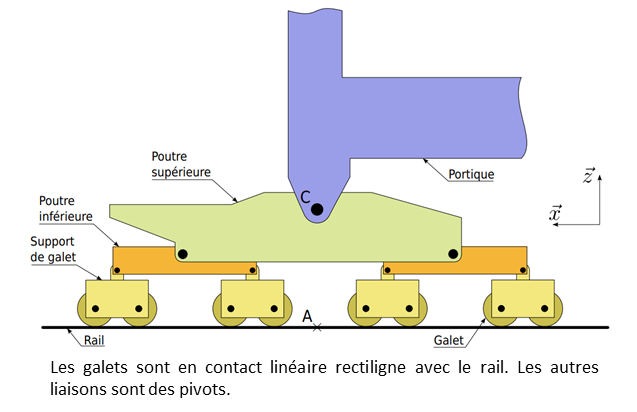
\includegraphics[width=5cm]{exo_05}
\end{center}
	\begin{reponses}	
	\bonne {12}
	\mauvaise 0
	\mauvaise 2
	\mauvaise 4
	\mauvaise 5
	\mauvaise 8
	\mauvaise {10}
	\end{reponses}
\end{question}\\}


 \element{mob2}{
 \begin{question}{mob2 6}
 Soit le schéma suivant. Donner la mobilité du mécanisme.
 \begin{center}
 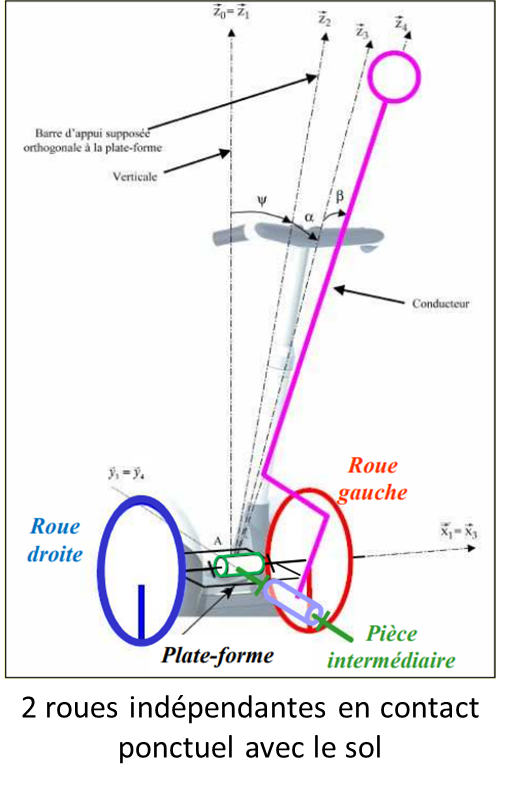
\includegraphics[width=5cm]{exo_06}
 \end{center}
	\begin{reponses}	
	\bonne 8
	\mauvaise 0
	\mauvaise 2
	\mauvaise 4
	\mauvaise 6
	\mauvaise 5
	\mauvaise 3
	\end{reponses}
 \end{question}\\}

 \element{mob2}{
 \begin{question}{mob2 7}
 Soit le schéma suivant. Donner la mobilité du mécanisme.
 \begin{center}
 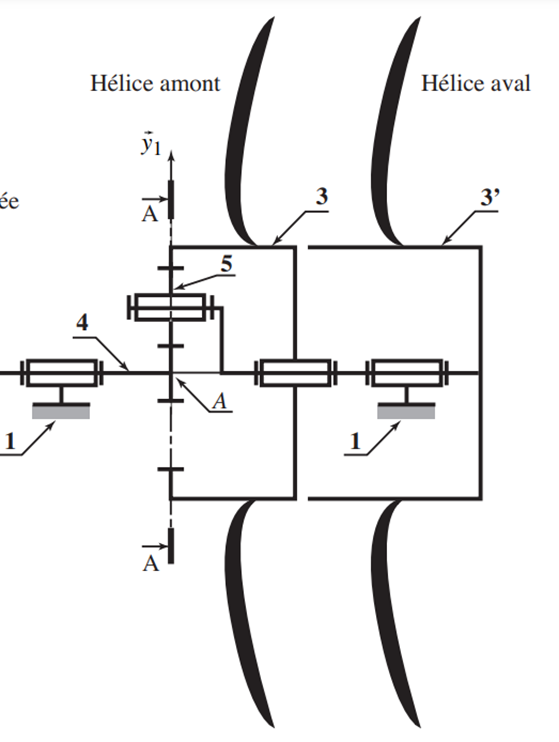
\includegraphics[width=5cm]{exo_07}
 \end{center}
	\begin{reponses}	
	\bonne 1
	\mauvaise 0
	\mauvaise 2
	\mauvaise 3
	\mauvaise 4
	\mauvaise 5
	\mauvaise 6
	\end{reponses}
 \end{question}\\}


 \element{mob2}{
 \begin{question}{mob2 8}
 Soit le schéma suivant. Donner la mobilité du mécanisme.
 \begin{center}
 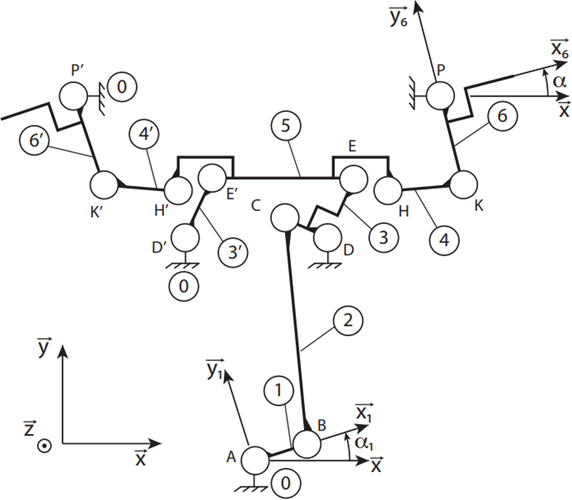
\includegraphics[width=5cm]{exo_08}
 \end{center}
	\begin{reponses}	
	\bonne 1
	\mauvaise 0
	\mauvaise 2
	\mauvaise 3
	\mauvaise 4
	\mauvaise 5
	\mauvaise 6
	\end{reponses}
 \end{question}\\}

 \element{mob2}{
 \begin{question}{mob2 9}
 Soit le schéma suivant. Donner la mobilité du mécanisme.
 \begin{center}
 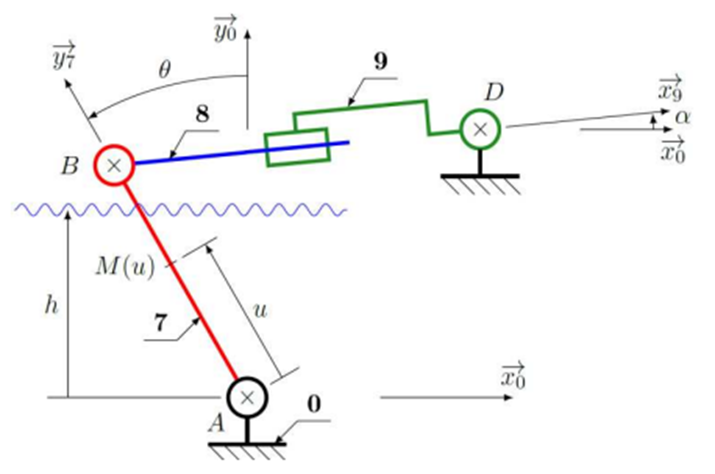
\includegraphics[width=5cm]{exo_09}
 \end{center}
	 \begin{reponses}	
	 \bonne 1
	 \mauvaise 0
	 \mauvaise 2
	 \mauvaise 3
	 \mauvaise 4
	 \mauvaise 5
	 \mauvaise 6
	 \end{reponses}
 \end{question}\\}

 \element{mob2}{
 \begin{question}{mob2 10}
 Soit le schéma suivant. Donner la mobilité du mécanisme.
 \begin{center}
 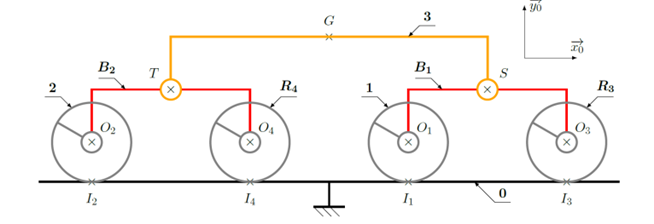
\includegraphics[width=5cm]{exo_10}
 \end{center}
	 \begin{reponses}	
	 \bonne 8
	 \mauvaise 0
	 \mauvaise 2
	 \mauvaise 4
	 \mauvaise 6
	 \mauvaise 5
	 \mauvaise 3
	 \end{reponses}
 \end{question}\\}

 \element{mob2}{
 \begin{question}{mob2 11}
 Soit le schéma suivant. Donner la mobilité du mécanisme.
 \begin{center}
 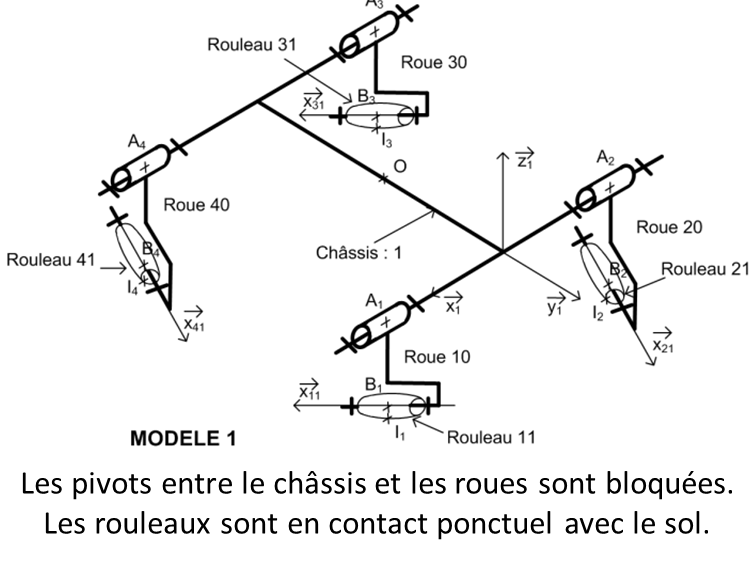
\includegraphics[width=5cm]{exo_11}
 \end{center}
	\begin{reponses}	
	 \bonne 7
	 \mauvaise 0
	 \mauvaise 2
	 \mauvaise 3
	 \mauvaise 4
	 \mauvaise 5
	 \mauvaise 6
	 \end{reponses}
 \end{question}\\}

 \element{hs}{
 \begin{question}{hs 01}
 Soit le schéma suivant. Donner le degré d'hyperstatisme du mécanisme.
 \begin{center}
 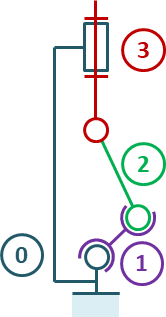
\includegraphics[width=3cm]{cas_01}
 \end{center}
	\begin{reponses}	
	\bonne 0
	\mauvaise 1
	\mauvaise 2
	\mauvaise 3
	\end{reponses}
 \end{question}\\}

 \element{hs}{
 \begin{question}{hs 02}
 Soit le schéma suivant. Donner le degré d'hyperstatisme du mécanisme.
 \begin{center}
 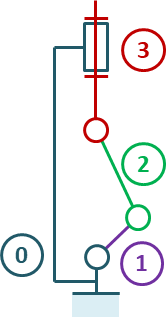
\includegraphics[width=3cm]{cas_02}
 \end{center}
	\begin{reponses}	
	\bonne 2
	\mauvaise 0
	\mauvaise 1
	\mauvaise 3
	\end{reponses}
 \end{question}\\}


 \element{hs}{
 \begin{question}{hs 03}
 Soit le schéma suivant. Donner le degré d'hyperstatisme du mécanisme.
 \begin{center}
 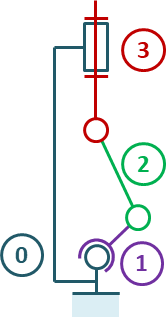
\includegraphics[width=3cm]{cas_03}
 \end{center}
	\begin{reponses}	
	\bonne 1
	\mauvaise 0
	\mauvaise 2
	\mauvaise 3
	\end{reponses}
 \end{question}\\}


 \element{hs}{
 \begin{question}{hs 04}
 Soit le schéma suivant. Donner le degré d'hyperstatisme du mécanisme.
 \begin{center}
 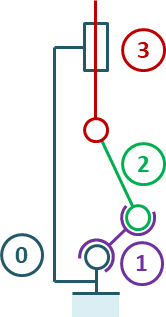
\includegraphics[width=3cm]{cas_04}
 \end{center}
	\begin{reponses}	
	\bonne 0
	\mauvaise 3
	\mauvaise 1
	\mauvaise 2
	\end{reponses}
 \end{question}\\}

 \element{hs}{
 \begin{question}{hs 05}
 Soit le schéma suivant. Donner le degré d'hyperstatisme du mécanisme.
 \begin{center}
 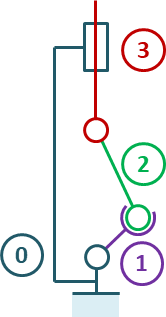
\includegraphics[width=3cm]{cas_05}
 \end{center}
	\begin{reponses}	
	\bonne 1
	\mauvaise 0
	\mauvaise 2
	\mauvaise 3
	\end{reponses}
 \end{question}\\}


 \element{hs}{
 \begin{question}{hs 06}
 Soit le schéma suivant. Donner le degré d'hyperstatisme du mécanisme.
 \begin{center}
 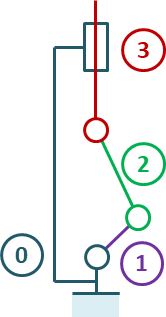
\includegraphics[width=3cm]{cas_06}
 \end{center}
	\begin{reponses}	
	\bonne 2
	\mauvaise 0
	\mauvaise 1
	\mauvaise 3
	\end{reponses}
 \end{question}\\}

 \element{hs}{
 \begin{question}{hs 07}
 Soit le schéma suivant. Donner le degré d'hyperstatisme du mécanisme.
 \begin{center}
 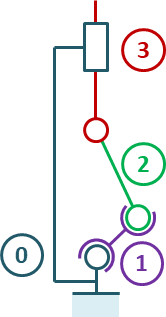
\includegraphics[width=3cm]{cas_07}
 \end{center}
	\begin{reponses}	
	\bonne 0
	\mauvaise 1
	\mauvaise 2
	\mauvaise 3
	\end{reponses}
 \end{question}\\}

 \element{hs}{
 \begin{question}{hs 08}
 Soit le schéma suivant. Donner le degré d'hyperstatisme du mécanisme.
 \begin{center}
 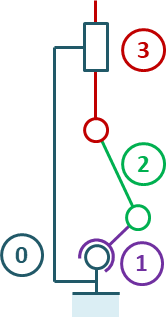
\includegraphics[width=3cm]{cas_08}
 \end{center}
	\begin{reponses}	
	\bonne 1
	\mauvaise 0
	\mauvaise 2
	\mauvaise 3
	\end{reponses}
 \end{question}\\}


 \element{hs}{
 \begin{question}{hs 09}
 Soit le schéma suivant. Donner le degré d'hyperstatisme du mécanisme.
 \begin{center}
 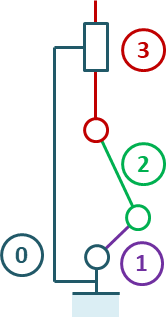
\includegraphics[width=3cm]{cas_09}
 \end{center}
	\begin{reponses}	
	\bonne 3
	\mauvaise 0
	\mauvaise 2
	\mauvaise 1
	\end{reponses}
 \end{question}\\}


 \element{hs}{
 \begin{question}{hs 10}
 Soit le schéma suivant. Donner le degré d'hyperstatisme du mécanisme.
 \begin{center}
 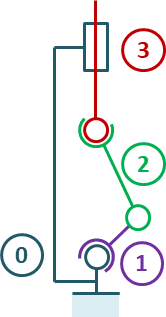
\includegraphics[width=3cm]{cas_10}
 \end{center}
	\begin{reponses}	
	\bonne 0
	\mauvaise 1
	\mauvaise 2
	\mauvaise 3
	\end{reponses}
 \end{question}\\}


 \element{hs}{
 \begin{question}{hs 11}
 Soit le schéma suivant. Donner le degré d'hyperstatisme du mécanisme.
 \begin{center}
 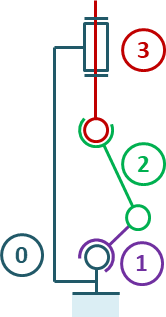
\includegraphics[width=3cm]{cas_11}
 \end{center}
	\begin{reponses}	
	\bonne 0
	\mauvaise 1
	\mauvaise 2
	\mauvaise 3
	\end{reponses}
 \end{question}\\}

 \element{hs}{
 \begin{question}{hs 12}
 Soit le schéma suivant. Donner le degré d'hyperstatisme du mécanisme.
 \begin{center}
 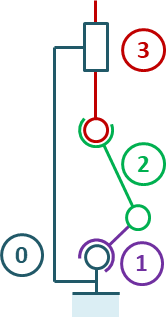
\includegraphics[width=3cm]{cas_12}
 \end{center}
	\begin{reponses}	
	\bonne 0
	\mauvaise 1
	\mauvaise 2
	\mauvaise 3
	\end{reponses}
 \end{question}\\}


 \element{hs2}{
 \begin{question}{hs2 1}
 Soit le schéma suivant. Donner le degré d'hyperstatisme du mécanisme.
 \begin{center}
 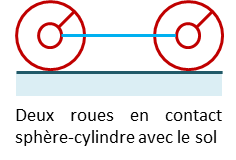
\includegraphics[width=5cm]{exo_01}
 \end{center}
	\begin{reponses}	
	\bonne 0
	\mauvaise 1
	\mauvaise 2
	\mauvaise 3
	\mauvaise 4
	\mauvaise 5
	\mauvaise 6
	\end{reponses}
 \end{question}\\}

 \element{hs2}{
 \begin{question}{hs2 2}
 Soit le schéma suivant. Donner le degré d'hyperstatisme du mécanisme.
 \begin{center}
 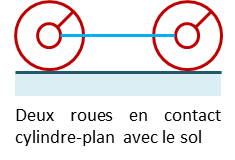
\includegraphics[width=5cm]{exo_02}
 \end{center}
	\begin{reponses}	
	\bonne 2
	\mauvaise 0
	\mauvaise 1
	\mauvaise 3
	\mauvaise 4
	\mauvaise 5
	\mauvaise 6
	\end{reponses}
 \end{question}\\}

 \element{hs2}{
 \begin{question}{hs2 3}
 Soit le schéma suivant. Donner le degré d'hyperstatisme du mécanisme.
 \begin{center}
 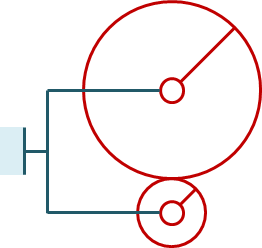
\includegraphics[width=5cm]{exo_03}
 \end{center}
	\begin{reponses}	
	\bonne 1
	\mauvaise 0
	\mauvaise 2
	\mauvaise 3
	\mauvaise 4
	\mauvaise 5
	\mauvaise 6
	\end{reponses}
 \end{question}\\}

 \element{hs2}{
 \begin{question}{hs2 4}
 Soit le schéma suivant. Donner le degré d'hyperstatisme du mécanisme.
 \begin{center}
 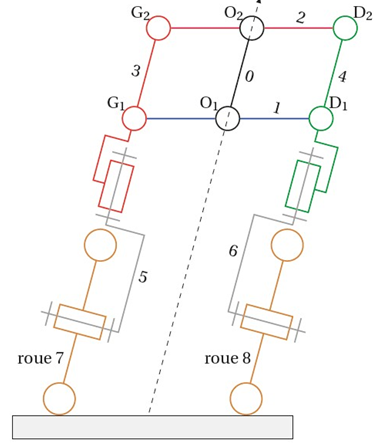
\includegraphics[width=5cm]{exo_04}
 \end{center}
	\begin{reponses}	
	\bonne 7
	\mauvaise 6
	\mauvaise 5
	\mauvaise 4
	\mauvaise 3
	\mauvaise 2
	\mauvaise 1
	\end{reponses}
 \end{question}\\}

 \element{hs2}{
 \begin{question}{hs2 5}
 Soit le schéma suivant. Donner le degré d'hyperstatisme du mécanisme.
 \begin{center}
 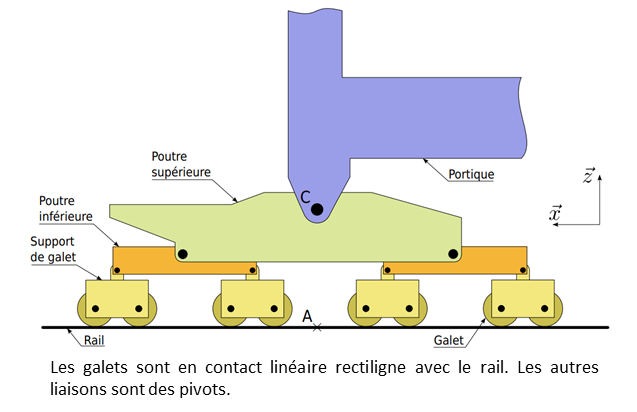
\includegraphics[width=5cm]{exo_05}
 \end{center}
	\begin{reponses}	
	\bonne 7
	\mauvaise 6
	\mauvaise 5
	\mauvaise 4
	\mauvaise 3
	\mauvaise 2
	\mauvaise 1
	\end{reponses}
 \end{question}\\}

 \element{hs2}{
 \begin{question}{hs2 6}
 Soit le schéma suivant. Donner le degré d'hyperstatisme du mécanisme.
 \begin{center}
 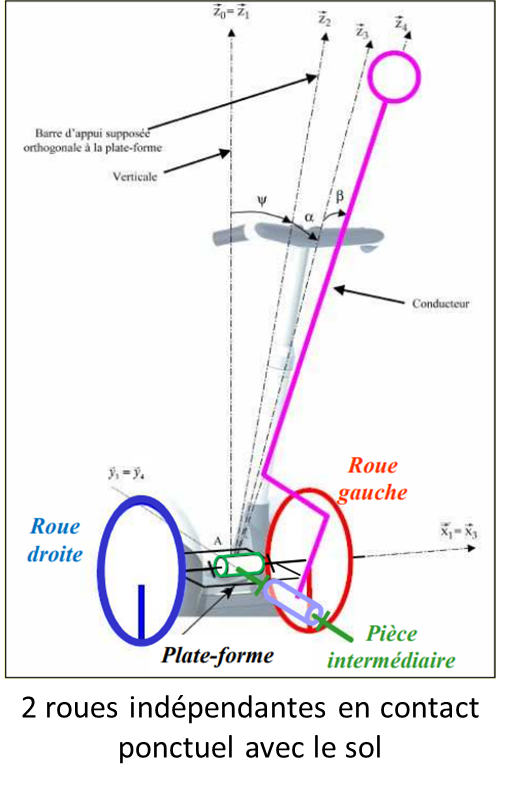
\includegraphics[width=5cm]{exo_06}
 \end{center}
	\begin{reponses}	
	\bonne 1
	\mauvaise 0
	\mauvaise 2
	\mauvaise 3
	\mauvaise 4
	\mauvaise 5
	\mauvaise 6
	\end{reponses}
 \end{question}\\}

 \element{hs2}{
 \begin{question}{hs2 7}
 Soit le schéma suivant. Donner le degré d'hyperstatisme du mécanisme.
 \begin{center}
 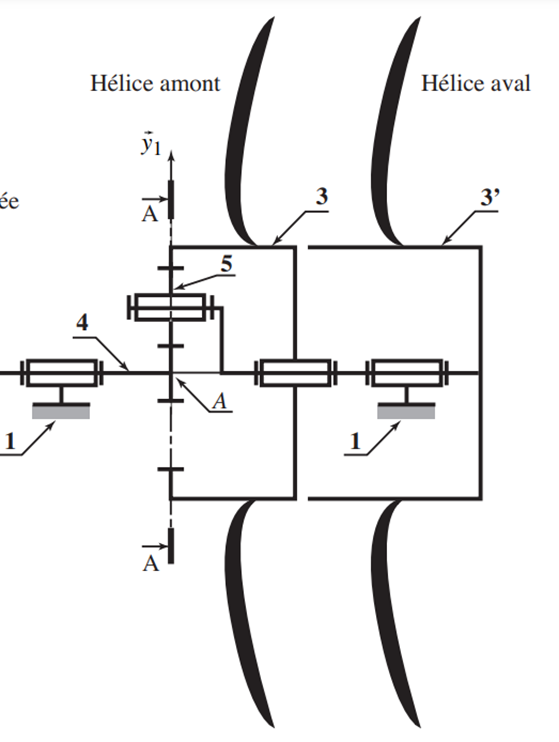
\includegraphics[width=5cm]{exo_07}
 \end{center}
	\begin{reponses}	
	\bonne 3
	\mauvaise 0
	\mauvaise 1
	\mauvaise 2
	\mauvaise 4
	\mauvaise 5
	\mauvaise 6
	\end{reponses}
 \end{question}\\}


 \element{hs2}{
 \begin{question}{hs2 8}
 Soit le schéma suivant. Donner le degré d'hyperstatisme du mécanisme.
 \begin{center}
 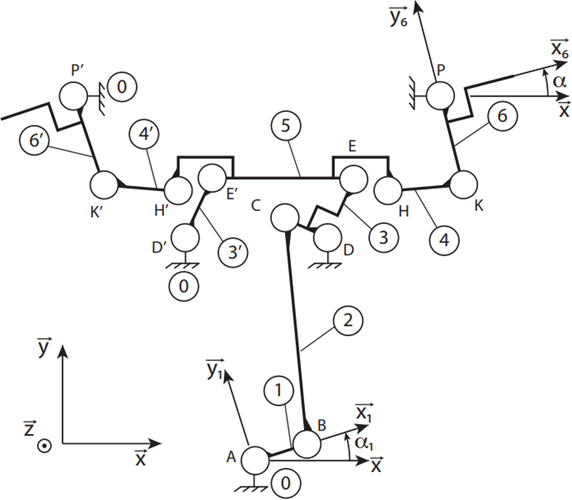
\includegraphics[width=5cm]{exo_08}
 \end{center}
	\begin{reponses}	
	\bonne {12}
	\mauvaise {10}
	\mauvaise 8
	\mauvaise 6
	\mauvaise 4
	\mauvaise 2
	\mauvaise 0
	\end{reponses}
 \end{question}\\}

 \element{hs2}{
 \begin{question}{hs2 9}
 Soit le schéma suivant. Donner le degré d'hyperstatisme du mécanisme.
 \begin{center}
 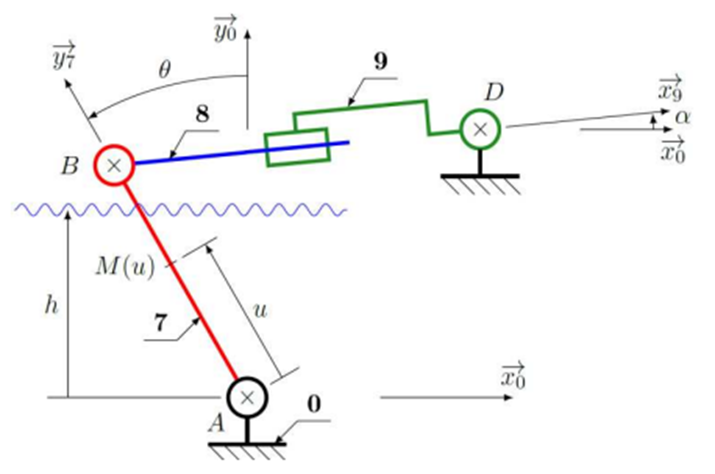
\includegraphics[width=5cm]{exo_09}
 \end{center}
	\begin{reponses}	
	\bonne 2
	\mauvaise 0
	\mauvaise 1
	\mauvaise 3
	\mauvaise 4
	\mauvaise 5
	\mauvaise 6
	\end{reponses}
 \end{question}\\}

 \element{hs2}{
 \begin{question}{hs2 10}
 Soit le schéma suivant. Donner le degré d'hyperstatisme du mécanisme.
 \begin{center}
 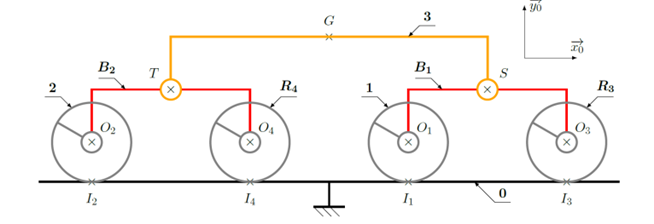
\includegraphics[width=5cm]{exo_10}
 \end{center}
	\begin{reponses}	
	\bonne 2
	\mauvaise 0
	\mauvaise 1
	\mauvaise 3
	\mauvaise 4
	\mauvaise 5
	\mauvaise 6
	\end{reponses}
 \end{question}\\}

 \element{hs2}{
 \begin{question}{hs2 11}
 Soit le schéma suivant. Donner le degré d'hyperstatisme du mécanisme.
 \begin{center}
 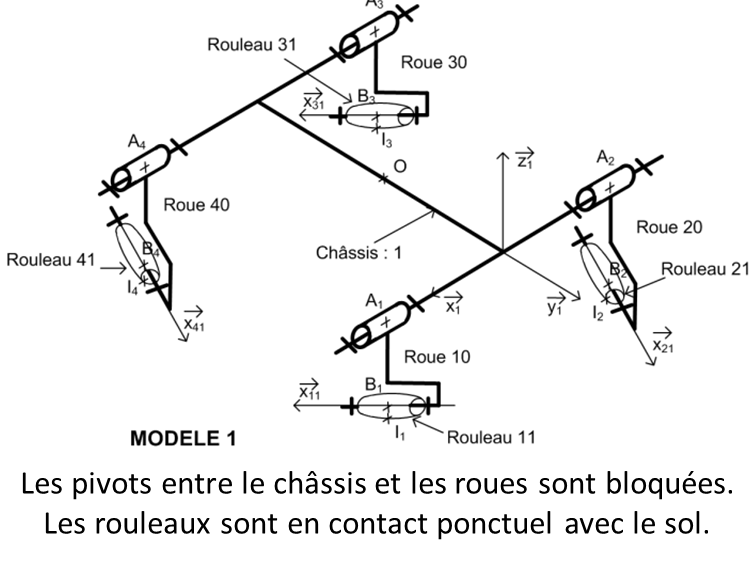
\includegraphics[width=5cm]{exo_11}
 \end{center}
	\begin{reponses}	
	\bonne 1
	\mauvaise 0
	\mauvaise 2
	\mauvaise 3
	\mauvaise 4
	\mauvaise 5
	\mauvaise 6
	\end{reponses}
 \end{question}\\}
